% JuliaCon proceedings template
\documentclass{juliacon}
\setcounter{page}{1}
\usepackage{amsmath}
\usepackage{cleveref}

% If using Emacs, put cursor on last closing paren and call "eval-last-sexp" (usually `C-x C-e') to regenerate
\iffalse
(save-excursion
  (let* ((toc (funcall imenu-create-index-function))
         (headers (mapcar (pcase-lambda (`(,str . ,loc)) str)
                          toc)))
    (beginning-of-buffer)
    (search-forward (concat "%% " "--- autogenerated TOC ---"))
    (next-line)
    (beginning-of-line)
    (let ((start (point)))
      (search-forward (concat "%% " "--- end autogenerated TOC ---"))
      (beginning-of-line)
      (delete-region start (point))
      (goto-char start))
    (cl-loop for header in headers
             do (insert (format "%% %s\n" header)))
    (next-line)))
\fi

%% --- autogenerated TOC ---
% juliacon
% document
%   Introduction
%   To Kill a Floating Point
%     Where do NaNs come from?
%     NaN kills
%   FloatTracker Internals
%     Catching NaN kills
%     NaN propagation monitoring
%     NaN injection
%   Case Studies
%     Surprise NaNs: ShallowWaters
%     NaN fuzzing to find a kill: OrdinaryDiffEq
%     Finch
%     A Bug-Hunting Safari
%   Evaluation
%   Discussion
%     Tracking more than NaNs
%     Enhanced Fuzzing
%   Related Work
%   Acknowledgments
% document
%% --- end autogenerated TOC ---

\begin{document}

% **************GENERATED FILE, DO NOT EDIT**************

\title{My JuliaCon proceeding}

\author[1]{Taylor Allred}
\author[1]{Xinyi Li}
\author[1]{Ashton Wiersdorf}
\author[1]{Ben Greenman}
\author[1]{Ganesh Gopalakrishnan}
\affil[1]{University of Utah}

\keywords{Julia, Optimization, Game theory, Compiler}

\hypersetup{
pdftitle = {My JuliaCon proceeding},
pdfsubject = {JuliaCon 2019 Proceedings},
pdfauthor = {1st author, 2nd author, 3rd author},
pdfkeywords = {Julia, Optimization, Game theory, Compiler},
}


\maketitle

\begin{abstract}
  Reliable numerical computations are central to high-performance computing and machine learning.
  We present FlowFPX: a Julia-based tool for tracking the onset and flow of IEEE Floating-Point exceptions that signal numerical defects.
  FlowFPX's design exploits Julia's operator overloading to trace exception flows and even inject exceptions to accelerate testing.
  We present intuitive visualizations of summarized exception flows including how they are generated, propagated and killed, thus helping with debugging and repair.
\end{abstract}

\newcommand{\code}[1]{\texttt{#1}}
\newcommand{\FlowFPX}{FlowFPX}
\newcommand{\FloatTracker}{FloatTracker}
\newcommand{\FT}{\FloatTracker}
\newcommand{\CSTG}{stack graph}
\newcommand{\CPP}{\code{C++}}
\newcommand{\Dendro}{\textsc{Dendro}}
\newcommand{\urlaccess}[2]{\url{#1}}

\section{Introduction}

\section{To Kill a Floating Point}
% If anyone has a better "kill" pun/reference than "To Kill a Mockingbird", I'm all ears.
% I think we will definitely need a clear, detailed section on how NaNs crop up and how they can be killed.

The IEEE 754 specification for floating-point numbers governs how NaNs are handled as arguments to arithmetic functions~\cite{IEEEStandardBinary1985}.
Most of the time, when any or all of the arguments are NaN, the result is also a NaN.
This is good and desirable, because it means that an arithmetic error---even if buried deep in an expression---will still be observable, allowing a user to find and debug it.

However, there are a few places where NaNs flow into an expression, but not out.
We call these instances ``NaN-kills'', and these can lead to subtle logic bugs.
Consider the following example:

\begin{lstlisting}[language = Julia]
function bad_max(lst)
  max_seen = 0.0
  for x in lst
    if ! (x <= max_seen)
      # swap if new val greater
      max_seen = x
    end
  end
  max_seen
end

function good_max(lst)
  foldl(max, lst)
end
\end{lstlisting}

Both \texttt{bad\_max} and \texttt{good\_max} compute the maximum in a list.
However, the \texttt{<=} operator used in the \texttt{bad\_max} implementation does \emph{not} propagate NaNs, so you might not get the result you expected:

\begin{lstlisting}[language = Julia]
bad_max([1, 5, NaN, 4])     # returns 4
good_max([1, 5, NaN, 4])    # returns NaN
\end{lstlisting}

Not only is the result from \texttt{bad\_max} problematic for obscuring the fact that there was a NaN in the list, the result is also wrong!
The built-in \texttt{max} function correctly propagates NaNs, so we can see from its return that we got a NaN somewhere.
It's not entirely obvious \emph{where} that NaN came from---but more on that later.   % this promise answered in "NaN propagation monitoring"

\subsection{Where do NaNs come from?}

IEEE 754~\cite{IEEEStandardBinary1985} lists the following operations (among a few others) where NaNs result:

\begin{figure}[h]
  \label{fig:nan-gens}
  \begin{itemize}
  \item $\frac{0}{0}$ or $\frac{\infty}{\infty}$
  \item $0 * \infty$
  \item $x \% y$ when $x = \infty$ or $y = 0$
  \item $+\infty + -\infty$ or $\infty - \infty$
  \item The square root or logarithm of a negative number
  \end{itemize}
  \caption{NaN-producing operations}
\end{figure}

% Yadda yadda yadda...

\subsection{NaN kills}

Most mathematical operations preserve NaNs.
However, there are some instances where NaNs can disappear, but not before potentially altering the correctness of the program!

% \begin{itemize}
% \item $x \; \texttt{cmp} \; y \rightarrow false$ where \texttt{cmp} is a binary comparison like \texttt{<}, \texttt{>}, \texttt{<=}, etc. and $x$ or $y$ is NaN.
% \item $1^{NaN} \rightarrow 1$
% \item $NaN^{0} \rightarrow 1$
% \end{itemize}

\begin{align*}
x \; \texttt{cmp} \; y &\rightarrow false &\text{where \texttt{cmp} is \texttt{<}, \texttt{>}, \texttt{<=}, etc.} \\
1^{\text{\texttt{NaN}}} &\rightarrow 1 \\
\text{\texttt{NaN}}^{0} &\rightarrow 1
\end{align*}

% Yadda yadda yadda...

% What else do we need to talk about? What other problems do we need to set up so that FloatTracker's solutions are clear?

\section{FloatTracker Internals}

FloatTracker works by leveraging Julia's type-based method dispatch system to capture everything from calls to the standard library down to basic arithmetic operations.
We do this by creating custom types \texttt{TrackedFloat16}, \texttt{TrackedFloat32}, and \texttt{TrackedFloat64} that wrap their corresponding \texttt{Float16}, \texttt{Float32} etc. counterparts.
We then defined methods for every function in the \texttt{Base} module, including new implementations for operators like \texttt{+} and \texttt{*}.
These new methods had to be defined for every combination of tracked/untracked arguments;
fortunately Julia's metaprogramming capabilities make this relatively simple.

The surrogate methods in place, every operation on a TrackedFloat can be intercepted.
We have three primary goals when intercepting a float:

\begin{enumerate}
  \item Catch instances of NaN kills
  \item Monitor the propagation of NaNs through the program
  \item Optionally \emph{inject} NaNs to fuzz the program under scrutiny against NaN-kills
\end{enumerate}

% Good things to put in this section:
% - start with the max example, perhaps?
% - trace examples
% - CSTGs
%
% Don't forget to talk about trace recording

\subsection{Catching NaN kills}

With a floating point value wrapped in our \texttt{TrackedFloat} type, it is easy to monitor when a NaN gets killed.
Julia dispatches all arithmetic operations on that value to flow through FloatTracker, where we can inspect the arguments.
Kills are relatively simple: if one or more NaNs flow into a function but don't flow out (i.e. the answer isn't a NaN) then that's a kill.
For example:

\begin{lstlisting}[language = Julia]
  NaN + 42     -> NaN    # not a kill
  Inf - Inf    -> NaN    # gen, but not a kill
  min(NaN, 42) -> NaN    # not a kill
  NaN < 42     -> false  # NaN kill!
\end{lstlisting}

There are a few exceptions to the rule of ``NaN in and no NaN out $\rightarrow$ kill''---some instances that we report as being a NaN kill might be instead a \emph{NaN-repair}, i.e. where the user explicitly checks for a NaN and gets some non-NaN value as a result.
Once clear instance of this is the \texttt{isnan} function.
Calling \texttt{isnan} and getting a boolean is expected behavior, and is usually used in error handling or in \emph{explicit} handling of unexpected values.
FloatTracker still reports these cases in the kill logs so as to be complete---the user must not blindly assume that every instance of a NaN kill is bad and might be a case of NaN repair.

% FIXME: we don't (yet) talk much about NaN repair in the rest of the paper.

% TODO?

\subsection{NaN propagation monitoring}

Remember in our first example with the \texttt{bad\_max} and \texttt{good\_max} functions how we didn't have a way to tell \emph{where} the NaNs originally came from?
That can be a tedious task.
However, FloatTracker makes this a lot easier by watching the life cycle of a NaN.

% TODO

% FIXME: don't forget to talk about CSTGs

\subsection{NaN injection}

% TODO

\section{Case Studies}

\FT{} is an effective tool for debugging all sorts of NaN-related issues.
We have used it to reveal silent NaNs, uncover the root cause of NaNs,
and fuzz for weak points in several case studies.


\subsection{Surprise NaNs: ShallowWaters}

Most physics simulations of this sort include a parameter called the Courant-Friedrichs-Lewy (``CFL'') parameter, which roughly describes the size of the time step to take in running the simulation.
Normally this value sits between 0 and 1---smaller values mean the simulation runs slower but with higher accuracy, whereas higher values mean the simulation takes bigger time steps and consequently runs faster, but results might be inaccurate.
The primary reason for problems arising comes from information not having enough time to propagate through the simulation before the next time step is taken.

It is not uncommon to encounter cases where setting the CFL parameter too high results in NaNs in the result.
Driving the CFL parameter low enough to excise the NaNs can make the simulation too long and unwieldy to be comfortable to use.
Identifying where NaNs begin to arise can help point the way to where some mathematical refinement can be used to make the simulation both fast and accurate enough for practical use.

For our first case study, we looked at the \texttt{ShallowWaters} library~\cite{klowerNumberFormatsError2020,klowerPositsAlternativeFloats2019,klowerLowprecisionClimateComputing2021}, which runs a simulates the flow of water over a seabed.
This is not a general shallow waters simulation library---it is designed primarily to showcase numerical methods involving 16-bit floats.
That said, it works for our purposes as a proving ground for FloatTracker.
We dialed the CFL parameter up to high values (as high as 10) and we started seeing NaNs in the result.
Note that the program did not crash: instead, it began producing bad output.

\begin{figure}
  \centering
  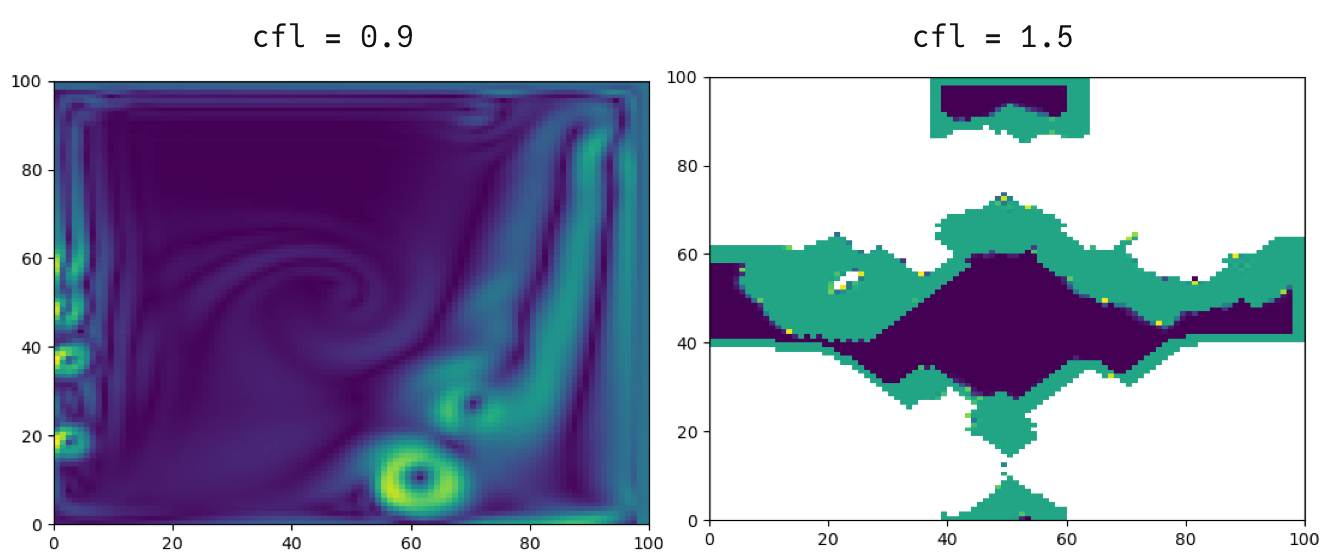
\includegraphics[width=3in]{./fig/shallow_waters_cfl_diff.png}
  \caption{Effect of high CFL parameters: on the left, normal output. On the right: NaNs cause white holes and gaps in the result.}
  \label{fig:sw_nans}
\end{figure}

The holes in the plots are regions where NaNs crept into the computation and destroyed the results.
In one regard, this is not as bad as a NaN kill---knowing that there are NaNs in the computation means that we have a chance to fix it, whereas a NaN kill might silently give us the wrong answer.
Incidentally, we know that there were no NaN kills in this test because our kill logs are empty.
But finding the sources of NaNs can be tricky.
We expected NaNs in this case because we set the CFL parameter up so high, but tracking down the sources of NaNs generally is a difficult and time-consuming problem.

Fortunately in this case, one of the key features \texttt{ShallowWaters} is its \emph{type flexibility}:
\texttt{ShallowWaters} was designed to showcase physics simulations using variable levels of floating-point precision.
Upon model construction, \texttt{ShallowWaters} allows you to specify a type for floats in the model.
We simply asked it to use our \texttt{TrackedFloat32} type, and then the entire simulation ran under the supervision of FloatTracker.

We ran ShallowWaters with a CFL value known to make bad outputs and recorded NaN \texttt{gen} events:

\begin{lstlisting}[language = Julia]
set_logger(buffersize=20, cstg=true, cstgArgs=true,
           cstgLineNum=true)

P = run_model(T=TrackedFloat32,
              cfl=10, Ndays=100, nx=100, L_ratio=1,
              bc="nonperiodic",
              wind_forcing_x="double_gyre",
              topography="seamount")
\end{lstlisting}

This produced the following in the log file: (formatted for clarity)

\begin{verbatim}
…
-                 FloatTracker/TrackedFloat.jl:106
momentum_u!       ShallowWaters/rhs.jl:246
rhs_nonlinear!    ShallowWaters/rhs.jl:50
rhs!              ShallowWaters/rhs.jl:14 [inlined]
time_integration  ShallowWaters/time_integration.jl:77
run_model         ShallowWaters/run_model.jl:37
…
\end{verbatim}

We can see that the NaN appeared from subtraction (first line) and that it was used in the \texttt{momentum\_u!} function on line 246 of the \texttt{rhs.jl} file (second line).
In figure~\ref{fig:nan-gens} we can tell that this must be the result of $\infty - \infty$.

Thus, with little effort we were able to track down where the NaNs were originating.
More work is needed to follow the $\infty$ back to wherever \emph{it} came from.
Fortunately, we will be able to extend FloatTracker to handle more than just NaNs---watching and logging \texttt{Inf}s should be completely tractable.
See~\cref{discussion} for more on future plans around this.

% TODO: if we get some handling with Inf working, then we should keep tracing this back.
% Where did the $\infty$ come from?

\subsection{NaN fuzzing to find a kill: OrdinaryDiffEq}

The second thing we evaluated was an N-Body simulation library.
We didn't find any sensible configuration of input parameters that lead to NaN kills like in the ShallowWaters library.
We turned to the NaN injection capabilities of FloatTracker to fuzz the library to find any lurking bugs.
% FIXME: add hyper-ref to § 4.1: ShallowWaters

We configured FloatTracker to inject a single NaN to see if we could find any NaN kills.
On some runs we noticed that we would get a kill and the program would warn about a NaN and prepare to exit.
Contrary to the error message's claim, however, the program went into an infinite loop.

The logs lead us to a routine in the widely-used \texttt{OrdinaryDiffEq} library.
During initialization, a NaN got injected during the execution of \texttt{-} between two \texttt{TrackedFloat}s:

\begin{verbatim}
…
-            at FloatTracker/src/TrackedFloat.jl:89
#__init#628  at OrdinaryDiffEq/src/solve.jl:106
…
\end{verbatim}

That injection point is here on third line of this snippet, which corresponds to line 106 from the \texttt{solve.jl} file in the \texttt{OrdinaryDiffEq} library:

\begin{lstlisting}[language = Julia]
tType = eltype(prob.tspan)
tspan = prob.tspan
tdir = sign(tspan[end] - tspan[1])

t = tspan[1]
\end{lstlisting}

\texttt{sign} correctly propagates NaNs, so \texttt{tdir} now contains a NaN.

We \emph{could} trace this variable through the code, but that would be a lot of grunt work.
Instead, we can look at the NaN kill logs to get a clue as to where we should look next:

\begin{verbatim}
…
<       at FloatTracker/src/TrackedFloat.jl:193
solve!  at OrdinaryDiffEq/src/solve.jl:515
…
\end{verbatim}

We get a very large kill file from this run, and the two lines from above show up repeatedly.
Thus, this is a good candidate location for where the cause of the loop is.

The relevant part of \texttt{solve.jl} looks like this:

% Note for Ashton:
% file here: ~/Research/ode_debug/dev/OrdinaryDiffEq/src/solve.jl
% see line 514

\begin{lstlisting}[language = Julia]
while !isempty(time_stops)
  while tdir * t < first(time_stops)
    # do integration work
  end
  pop_if_work_done(time_stops)
end
\end{lstlisting}

The problem here is on line 2 when \texttt{tdir} is NaN: multiplication propagates NaNs, and comparison kills it, so the condition on the inner \texttt{while} loop is \emph{always} false.
No work got done in the inner loop, and so the conditional \texttt{pop} routine never reduced the size of the \texttt{time\_stops} vector.

Our kill logs led us right to this line; this is a perfect example of how NaN kills can influence control flow to go awry.
In this case, the problem was apparent besides what our logs told us and it manifested as an infinite loop.
More dangerous cases can occur when the influence of a bad comparison is not as readily observable.

\subsection{Finch}
\label{s:finch}

Finch is a domain-specific language for specifying
PDEs~\cite{heislerFinchDomainSpecific2022}.\footnote{Not to be confused
with the Finch loop optimizer~\cite{adka-cgo-2023}.}
In the spirit of FEniCS~\cite{fenics} and related
tools~\cite{freefem,openfoam,dune,firedrake},
Finch helps scientists quickly convert math into code.
What sets Finch apart is its flexibility.
It supports multiple discretization methods (finite element and finite
volume) and multiple backends (Julia, \CPP{}, \Dendro{}~\cite{dendro}).
Furthermore it strives to output code that humans can easily fine-tune.

Fuzzing with \FT{} revealed two places where Finch needed
protection against user input.
The first was when reading an input mesh.\footnote{\urlaccess{https://github.com/paralab/Finch/issues/16}{2023-06-06}}
A NaN injected in the mesh led to a crash further on:
\begin{verbatim}
  BoundsError: attempt to access 1-element
   Vector{Int64} at index [2]
\end{verbatim}
Defensive programming solves the issue.
The second place was in setting bounds for the
solver.\footnote{\urlaccess{https://github.com/paralab/Finch/issues/17}{2023-06-06}}
Here, a NaN could leave bounds uninitialized, leading to a bounds error.
Additionally, \FT{} and \CSTG{}s have been useful for identifying NaNs that
appear in unstable systems.
%% advection2d, high cfl and high T (time) led to NaN during simulation


\subsection{A Bug-Hunting Safari}

% Notes on RxInfer

We searched GitHub for open issues in Julia libraries involving difficult-to-find NaNs.
In our first batch of issues, we found the \code{RxInfer.jl} library with an issue revolving around NaN detection.\footnote{\url{https://github.com/biaslab/RxInfer.jl/issues/116}}
We offered our tool for the package authors to use, and within a day the authors were able to track down the location of a NaN and fix the issue---all with minimal guidance.

\section{Evaluation}

\section{Discussion}
\label{s:discussion}

\subsection{Tracking more than NaNs}

% This is mostly a stand-in in case we don't get around to adding Inf tracking.
% It should be easy to do, but whether or not we have enough time to do it is
% another matter.
FloatTracker is capable of monitoring all sorts of events in a floating point value's lifetime---not just a value going to NaN.
Extending FloatTracker to handle \texttt{Inf} is just a matter of engineering.
Other values of interest may follow.

\subsection{Enhanced Fuzzing}

While fuzzing is useful for discovering issues, its success rate
is low because \emph{every} floating-point operation is a candidate
for injection.
Even operations that are already well-defended against NaNs are candidates.
\FT{} could use two sorts of tools for improving injection.
First, fine-grained control to let users decide where not to inject.
Second, tools for understanding the context of an injection point
after the fact.
Program slicing is especially relevant to the latter point (and effectively
what we did by hand when fuzzing Finch~\cref{s:finch}).
For each operation, an expert needs to study the values that feed into it to
decide whether they are protected or not.

%% TODO example, start here at glbvertex https://github.com/paralab/Finch/blob/master/src/grid.jl#L360


\section{Related Work}

\section{Acknowledgments}

We would also like to thank the developers of \code{RxInfer.jl} for feedback on \FlowFPX{}.

% **************GENERATED FILE, DO NOT EDIT**************

\bibliographystyle{juliacon}
\bibliography{ref.bib}


\end{document}

% Below is some Emacs-specific stuff. If you're using Emacs, you should try
% using the new jinx package for spell-checking!

% Local Variables:
% jinx-local-words: "CFL CSTGs Courant Friedrichs JuliaHub Lewy OrdinaryDiffEq RxInfer ShallowWaters TrackedFloat isnan"
% End:
